\section{Phase 2: Low Fidelity Prototype}
We used the results from our preliminary survey to inform our initial design work. Our focus on AR allowed us to explore how critical factors of online experiences from the original survey, such as access to reviews, could be brought into the store environment while preserving critical aspects of in-store decision making, such as being ``hands-on with the product'' and ``leaving the store with the product.'' 
%\todo{DNS: Is there a quote that can go here? MW: This is a quote from our early survey. Is it worth including/does it need to be cited? I could also dig something up from a related paper.}


\begin{marginfigure}
	\begin{minipage}{\marginparwidth}
			\centering
			\subfloat[][Context-aware paper prototype]{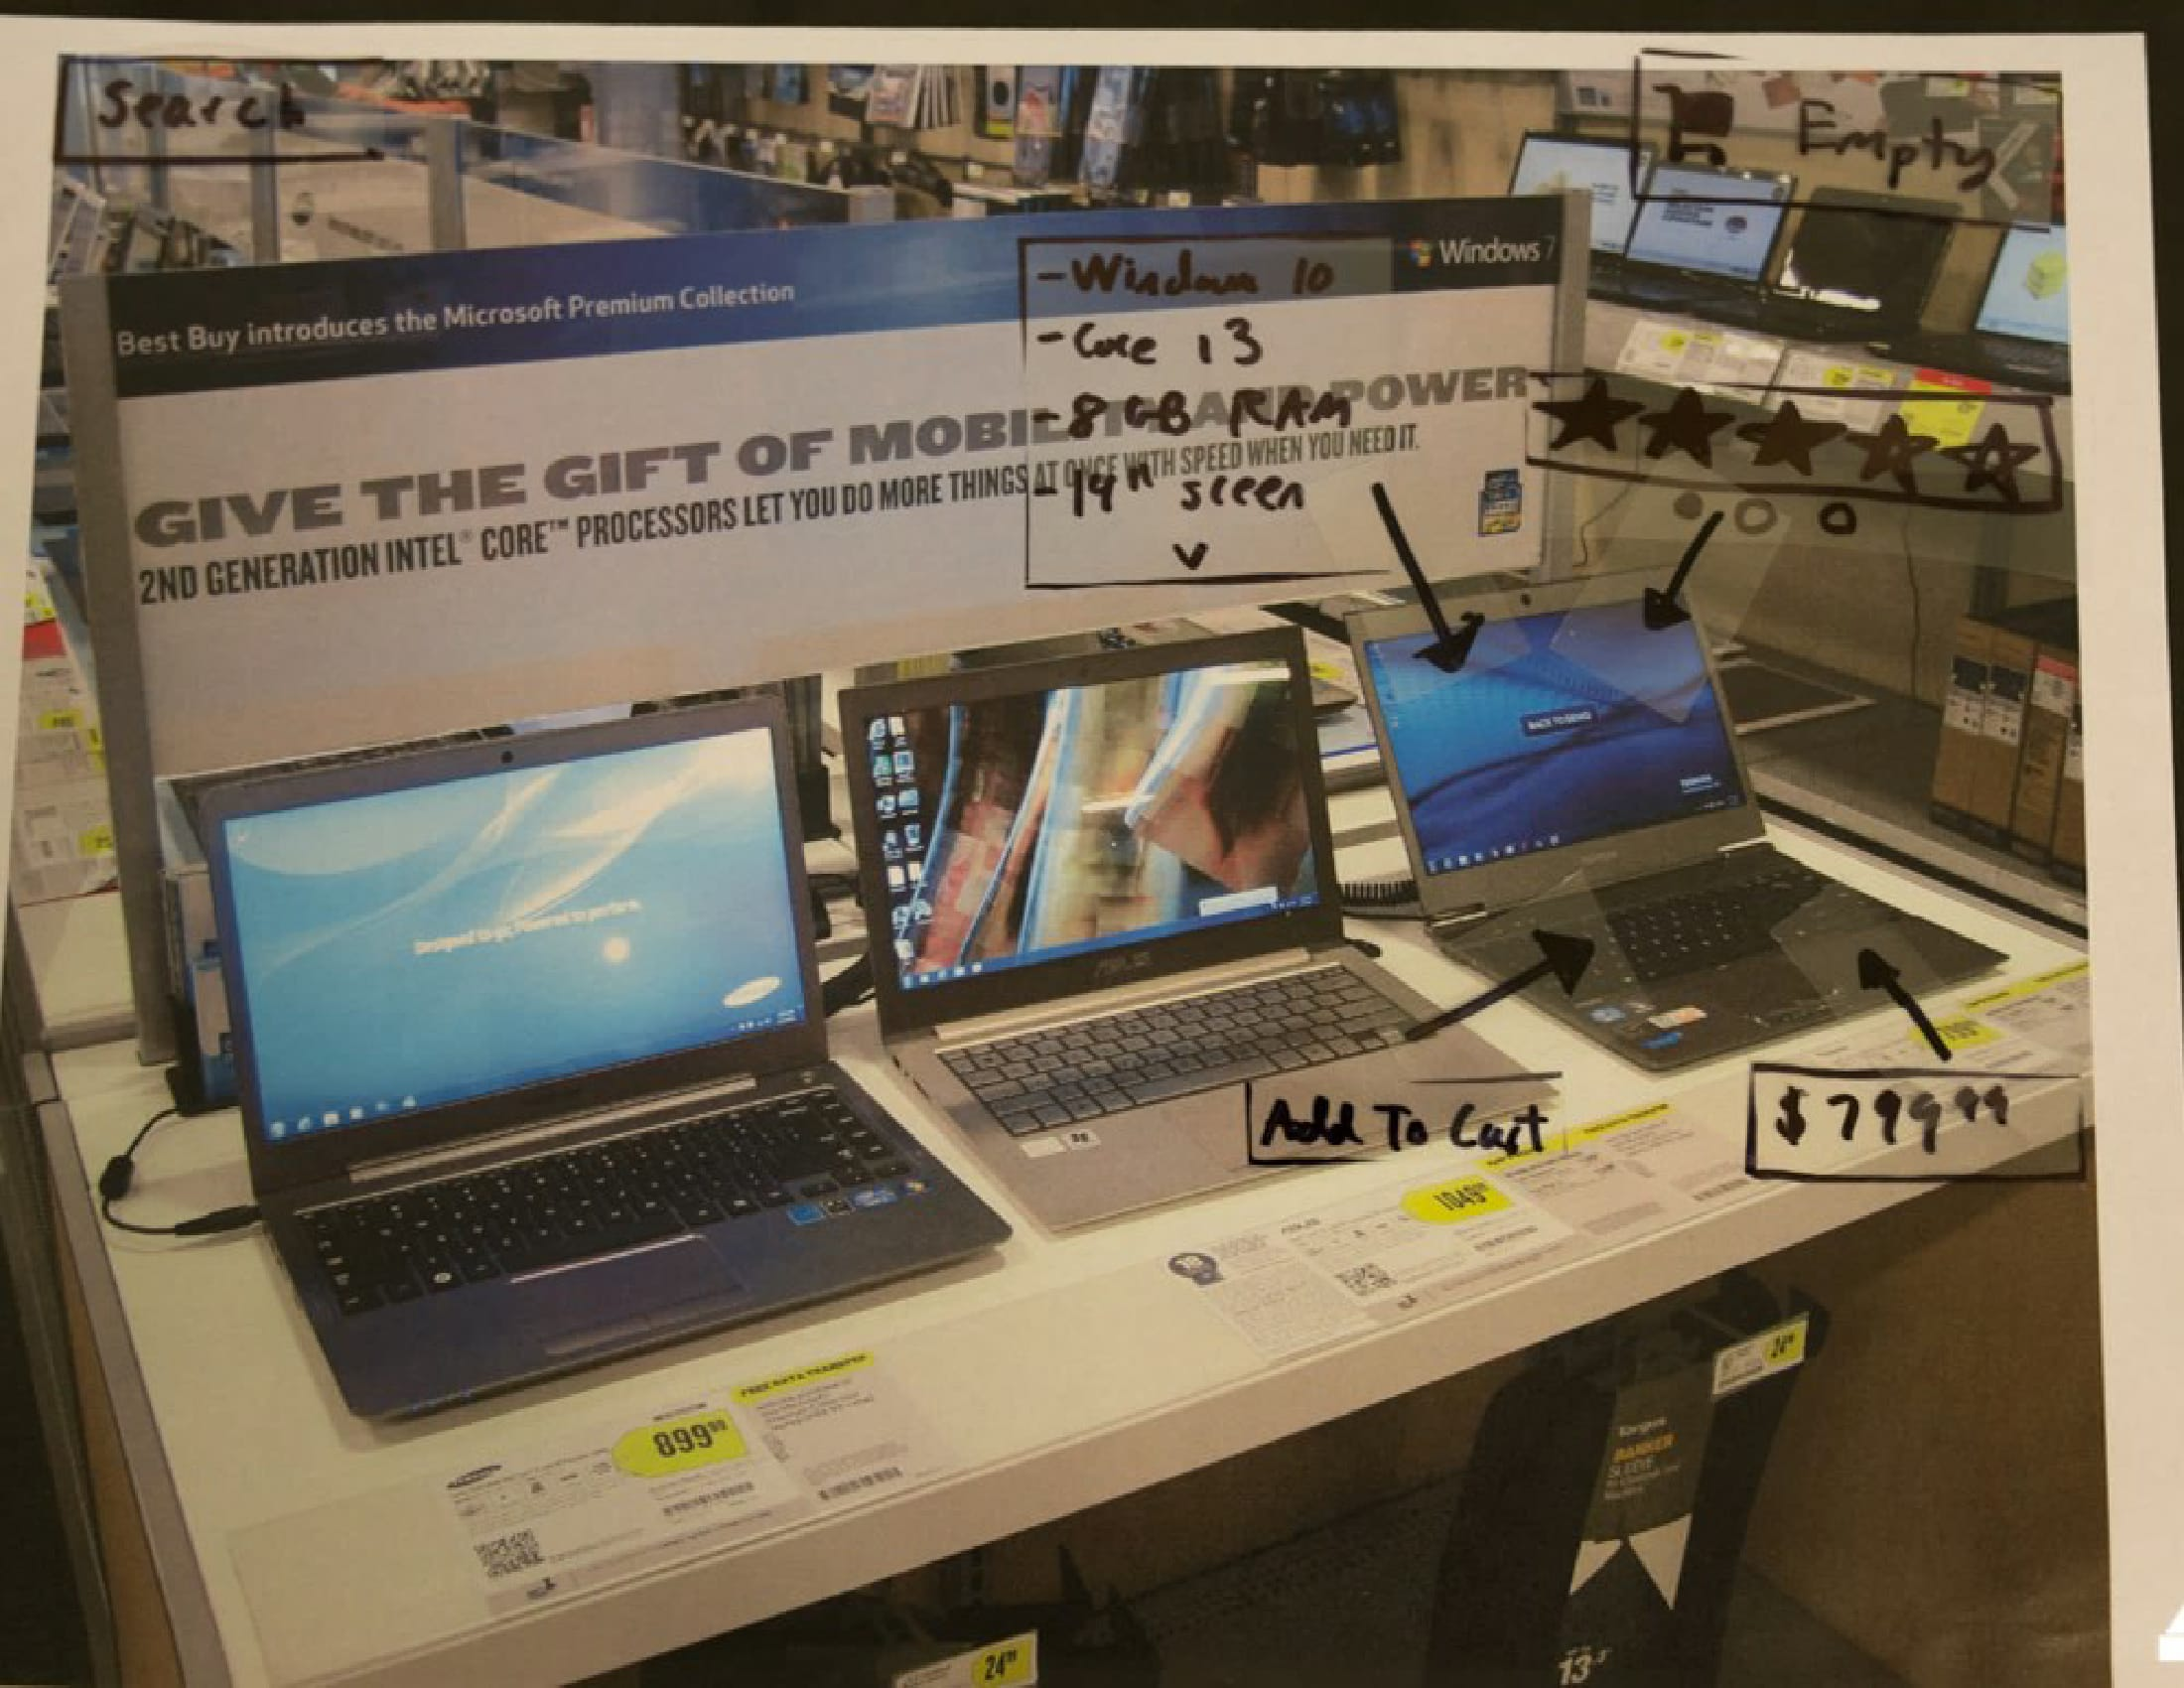
\includegraphics[width=0.9\columnwidth]{figures/LowFiContext}~\label{fig:LowFiContext}}
			\vfill
			\subfloat[][Menu-based paper prototype]{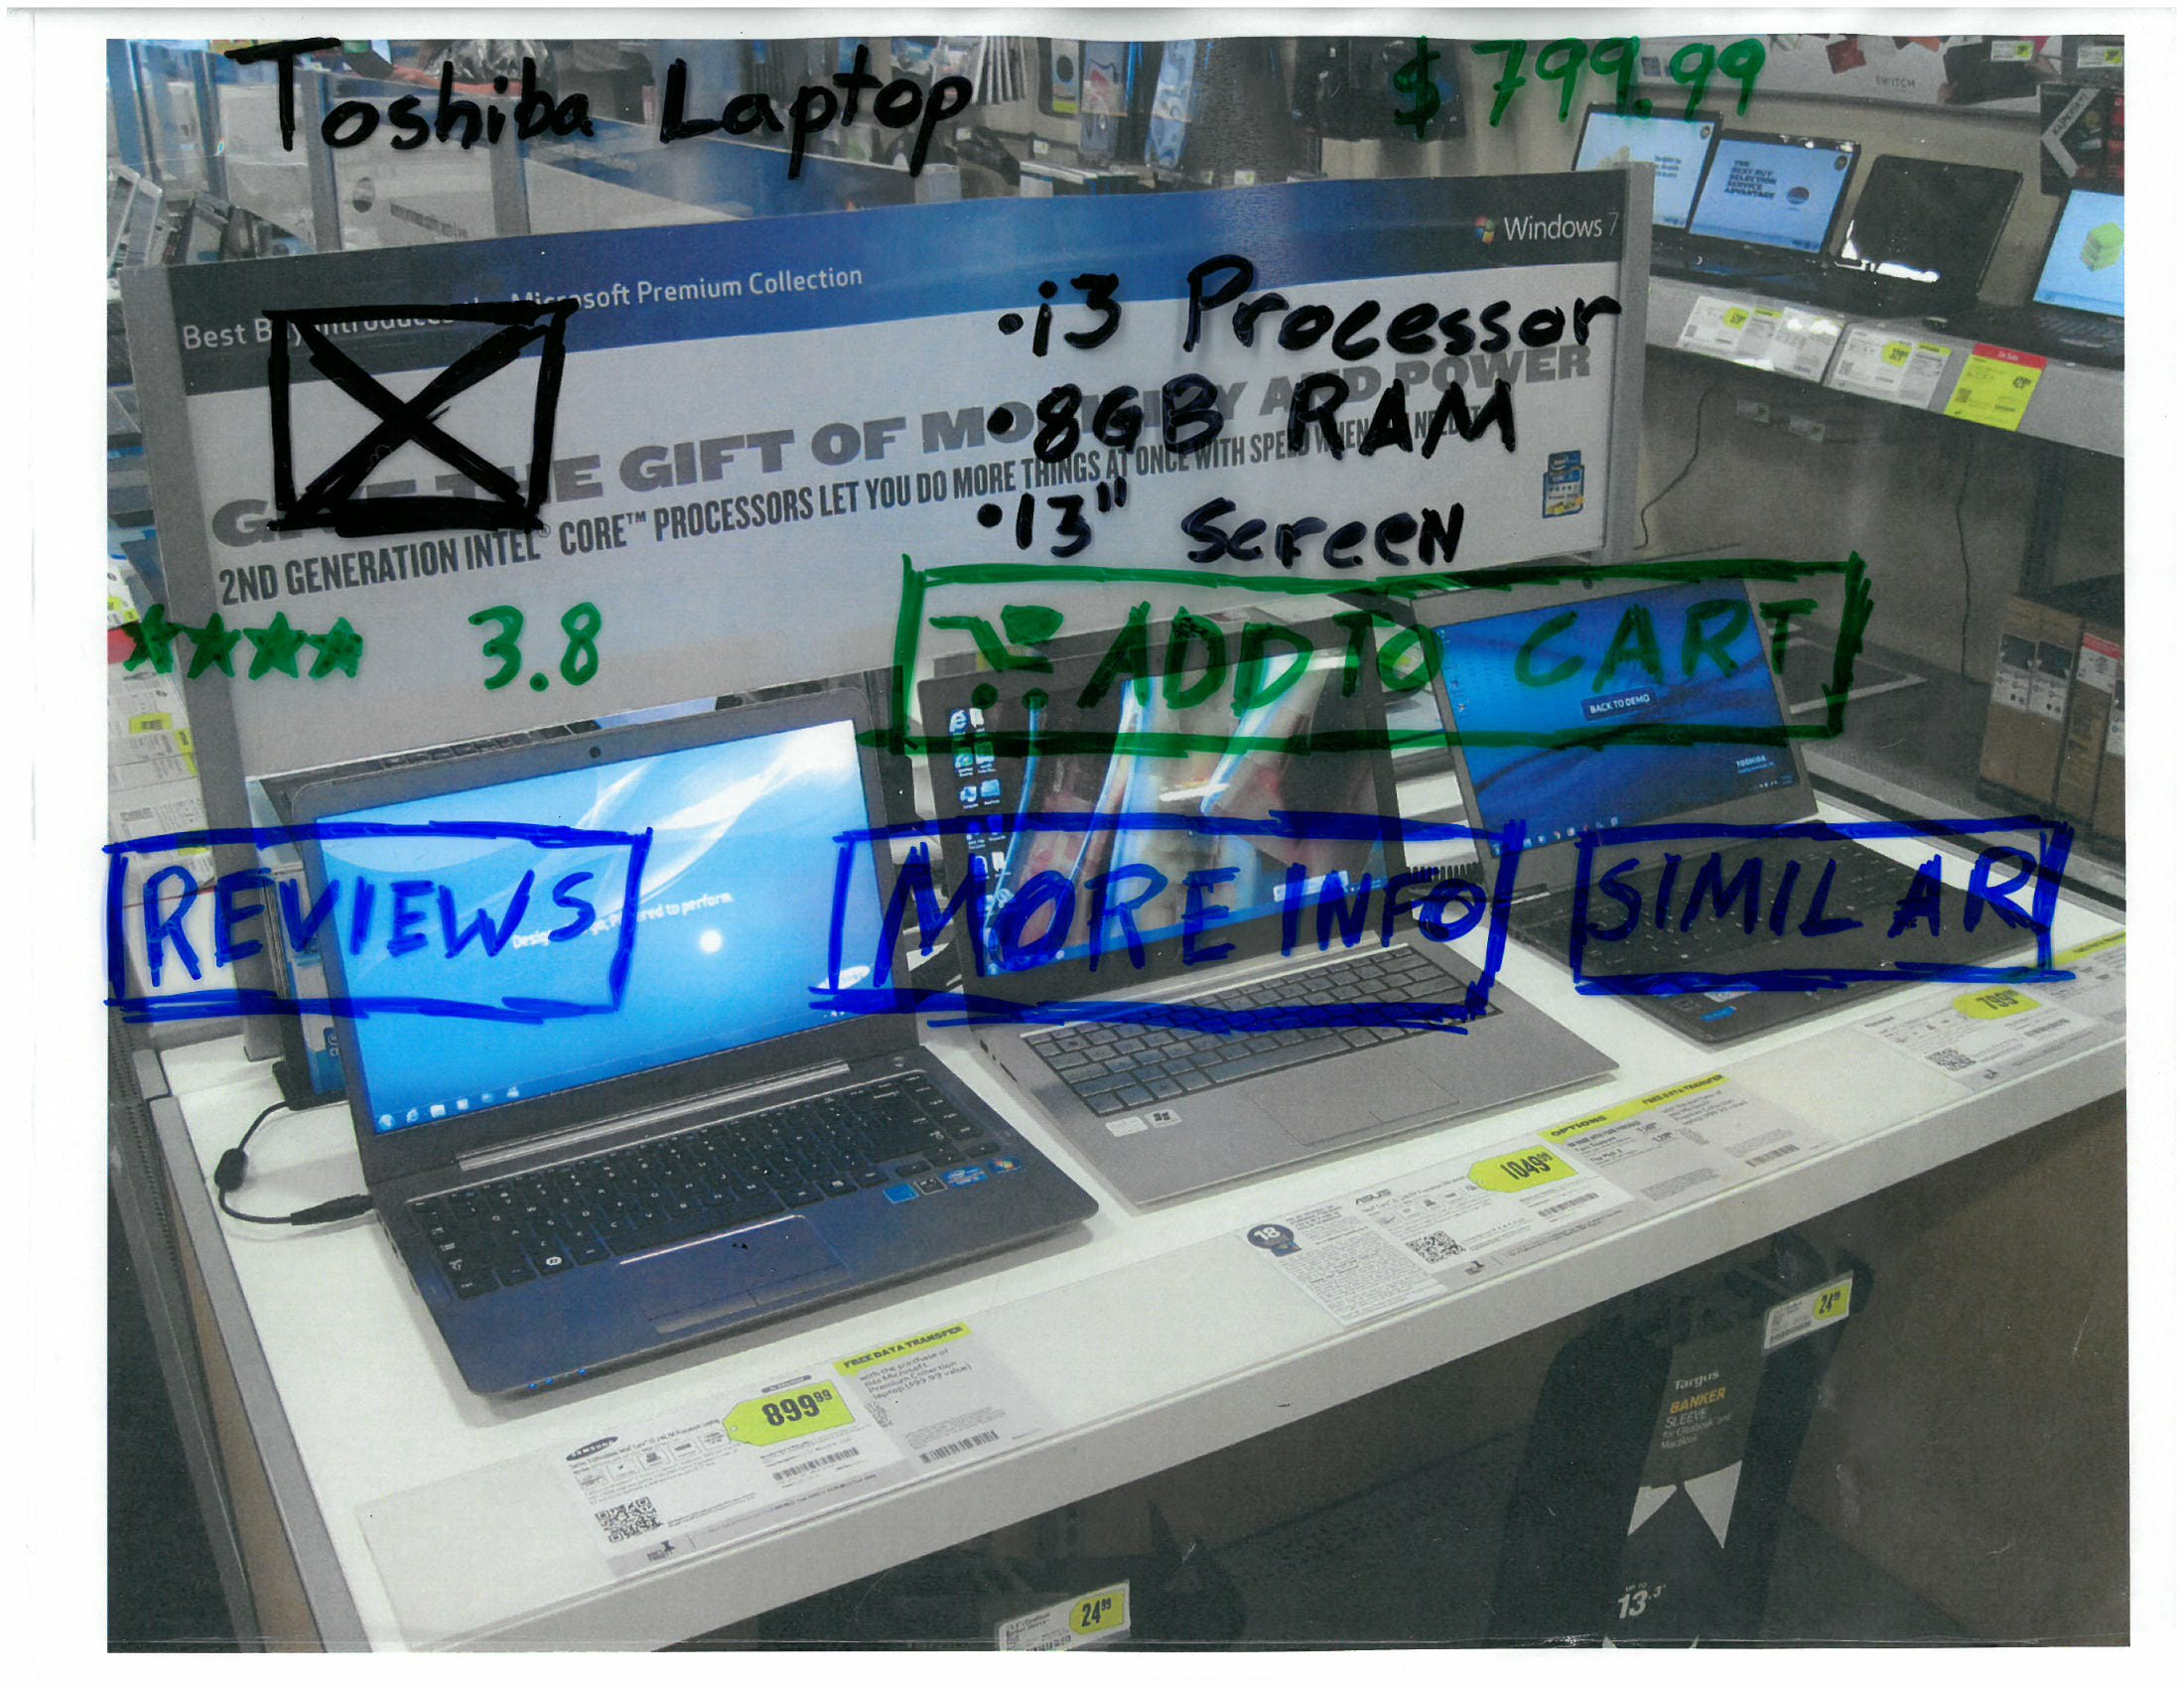
\includegraphics[width=0.9\columnwidth]{figures/LowFiMenu}~\label{fig:LowFiMenu}}
		\caption{Phase Two compared perceptions of a context-based and menu-based approach to augmenting traditional retail shopping with important factors of online shopping identified by participants in Phase One. }
	\end{minipage}
\end{marginfigure}

%\todo{replace the last bit of this sentence with what was actually tested} \todo{JRB: This sentence needs to be integrated once the correct content is put in there.} 
We used the results from our survey to design two sketch-based low fidelity prototypes of an AR system. 
%The layout and information content of our prototype reflected Phase One participants' most critical factors for  in-store and online shopping experiences. 
The prototypes, shown in Figures \ref{fig:LowFiContext} and \ref{fig:LowFiMenu}, consisted of online content drawn as AR menus on transparency sheets and overlaid onto an image of an electronics store. 
We used the prototypes to compare hierarchical menu-based content and context-aware virtual overlays for accessing information about price, review, rating, and product specifications. We collected feedback on our designs through a think-aloud with three participants.
% study using our sketch-based prototypes as a design prompt. \todo{JRB: Formative design work and evaluation do not have to be hypothesis driven, and often aren't. Instead they are exploratory. If you are feeling encumbered by the "hypothesis" language, we can reword. Just let me know.} 

Participants were asked to choose which laptop they would purchase for each condition based on the available information, with system type randomly ordered. 
% \todo[inline]{what specific AR components were tested here (e.g., reviews, product comparisons, specs, etc.)? What were your measures here (e.g., confidence in the decision, time to decision, etc.) MW: Briefly explained that in previous sentence} \todo{JRB: How did you analyze the data from this phase? MW: In English: We listened to them talk out loud and they told us how they are using the system in decision-making.} 
They walked us through the factors in their decision making processes, including how they would use each prototype in making their decision and absent features that would help formulate the decision. We recorded these responses and used them to inform the next phase of our work. 
%We recorded 
%user feedback as participants navigated the two systems. Our focus was on 
%qualitative responses informing us how this system helped them make a purchase decision.

Generally, participants were more receptive to concise information in the overlays than to the navigation-heavy menus. Participants felt the overlay was less obtrusive, better contextualized in the physical location of the products, and required less interaction to retrieve the necessary information. Participants felt that this would lead to faster and more confident decisions than a menu-based approach. 
%The unobtrusive nature and location-sensitive, quick information, and fewer interactions required provided by the context-aware prototype allowed for faster decision-making and increased understanding of the system's capabilities. \todo{JRB: Why? DNS--And how does this fit in with the design for Phase Three? MW: Basically, they weren't confused and did things faster} 
Participants also requested the ability to compare information about multiple products in one view, to toggle the displayed content, and to engage with visual product demonstrations for increased efficiency and more empowered decision making.

%DNS--Taking a stab at it
While our online survey suggested that people wanted access to more information, the paper prototype study enabled participants to envision the system in more detail and allowed us to identify how in-store and online experiences could be merged beyond simply taking the best features from each. For example, rather than simply more informaion and reviews, we found that participants wanted concise visual summaries of product ratings and specs. Simulated product demonstrations would leverage hands-free viewing to provide consumers with a tailored, hands-on experience in-store. 
We used these findings to 
%Our findings from the first two phases informed how we would approach the third phase of the design process. For the final prototype, we 
synthesize design features from that balance the important aspects of virtual and physical experiences while also considering the trade-offs of AR platforms in retail environments. 
%empower the user with important aspects of the virtual experience without sacrificing key aspects of the physical one. 
We did this by designing a context-aware approach to content delivery in the final phase of our design process. 
%\todo{JRB: This is a list of what they told you. Can you take it one step further and tell us what this means? What are the implications of these comments? You said you did this -- "We explored how understanding the trade-offs of parallel physical and virtual experiences could inform mixed reality applications in the context of retail shopping." -- so tell me what the results of this phase told you about those trade-offs. MW: I think this is what you had in mind}
